\subsection{Planificación de trayectorias}
\label{planificacion}

La planificación de trayectorias toma como entrada toda la información obtenida a través del algoritmo de procesamiento de imágenes: el mapa del entorno, la posición inicial del robot y la posición del objetivo, la lata.\\

El algoritmo elegido para la planificación de la ruta es un Quasi-Randomized Probabilistic Roadmap (Q-PRM), una variante del PRM que utiliza una distribución cuasi-aleatoria de puntos para calcular la hoja de ruta.\\

El algoritmo PRM tiene dos fases principales. En la primera, se genera el PRM propiamente dicho mediante un muestreo del espacio libre a través de una distribución aleatoria de puntos, que se conectan siguendo un criterio de distancias, procurando siempre que , tanto los nodos generados como las aristas que los conectan se encuentren en el espacio libre (no exista colisión con obstáculos. En la segunda, se realizan peticiones de caminos al mapa, conectando un punto inicial y uno final al grafo y calculando el camino más corto mediante un algoritmo de búsqueda en grafos, tal como el Djisktra o el $A^*$.\\

La mejora introducida por la variante Q-PRM es el uso de una distribución de puntos cuasi-aleatoria en lugar de aleatoria, lo que permite elegir una distribución de puntos que rellene el espacio de forma más óptima, siguiendo unos criterios de discrepancia y dispersión. \\

La discrepancia para un conjunto P formado por N muestras de d-dimensiones en $[0,1]^{d}$  viene dada por la ecuación \ref{eq:discrepancia}:
\begin{equation}
\label{eq:discrepancia}
D_N(P) = \sup_{j}{\left| \frac{A(J)}{N} -  \mu(J) \right| }
\end{equation}~\\

Donde J es cualquier subconjunto n-rectangular perteneciente a $[0,1]^{d}$, $\mu(J)$ es su medida n-dimensional y A(J) es el número de puntos que pertenecen a la unión entre P y J. En cuanto a la dispersión, hace referencia a la máxima distancia a la que cada punto de un conjunto puede estar respecto al punto mas cercano perteneciente a la misma secuencia. Por lo general, los conjuntos de puntos que presentan una baja discrepancia también poseerán una baja dispersión.\\

Estas distribuciones de puntos tienen la ventaja de ocupar el espacio libre de forma más eficiente, por lo que con menos cantidad de puntos se puede abarcar un área mayor y, por tanto, más partes delicadas del mapa. Estas partes delicadas pueden ser, por ejemplo, estrechamientos del espacio libre entre obstáculos.\\


Para el muestreo de puntos cuasi-aleatorios se han usado dos distribuciones de puntos: el conjunto de Hammersley y el conjunto de Halton. Estas distribuciones se generan a partir de una semilla para un número arbitrario de dimensiones. Estas distribuciones se pueden calcular de la siguiente manera:
\begin{itemize}
\item \textbf{Conjunto de Hammersley}: Dados $d-1$ números primos distintos $p_1, p_2, ... , p_{d-1}$ el i-ésimo punto del conjunto es dado por la expresión:
\[ \left( \frac{i}{N}, r_{p_1}(i), ..., r_{p_{d-1}(i)} \right), \qquad i = 0, 1, ..., N-1\]

\item \textbf{Conjunto de Halton} Dados $d$ números primos distintos $p_1, p_2, ..., p_d$ el i-ésimo punto del conjunto es dado por la siguiente expresión:
\[ \left( r_{p_1}(i),  r_{p_2}(i), ...,  r_{p_d}(i) \right) \]

\end{itemize}~\\

En ambos casos, la función $r_p(i)$ se obtiene  escribiendo los dígitos de la notación basada en $p$ en orden inverso. Por ejemplo, para la expresión $i = a_0 + a_1 p + a_2 p^2 + a_3 p^3 + ... $ donde $a_j \in \left\lbrace 0, 1, ... , p-1 \right\rbrace$ la función $r_p(i)$ sería:\\

\[ r_p(i) = \frac{a_0}{p} + \frac{a_1}{p^2} + \frac{a_2}{p^3} + \frac{a_3}{p^4} + ...\]\\

Para la implementación, se ha usado una biblioteca ya existente, perteneciente al paquete cgkit que proporciona estos conjuntos de puntos de manera cómoda y rápida, ahorrando tiempo de desarrollo y depuración de errores. La figura \ref{fig:muestreo} muestra una comparativa de los distintos métodos de generación de puntos de muestreo en un escenario ficticio.\\

\begin{figure}[h]
		\centering
        \begin{subfigure}[b]{0.3\textwidth}
                \centering
                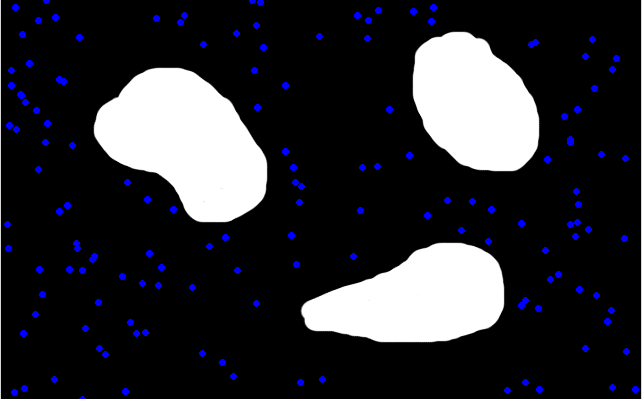
\includegraphics[width=\textwidth]{images/random.png}
                \caption{Muestreo aleatorio}
                \label{fig:muestreo_aleatorio}
        \end{subfigure}
        ~
        \begin{subfigure}[b]{0.3\textwidth}
                \centering
                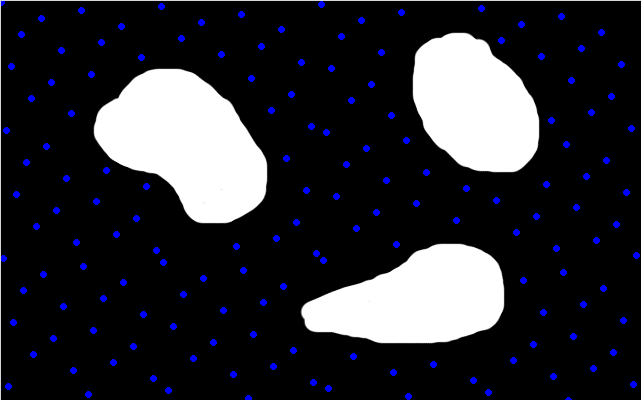
\includegraphics[width=\textwidth]{images/hammersley.png}
                \caption{Muestreo con puntos Hammersley}
                \label{fig:muestreo_hammersley}
        \end{subfigure}
        ~
        \begin{subfigure}[b]{0.3\textwidth}
         	   \centering
                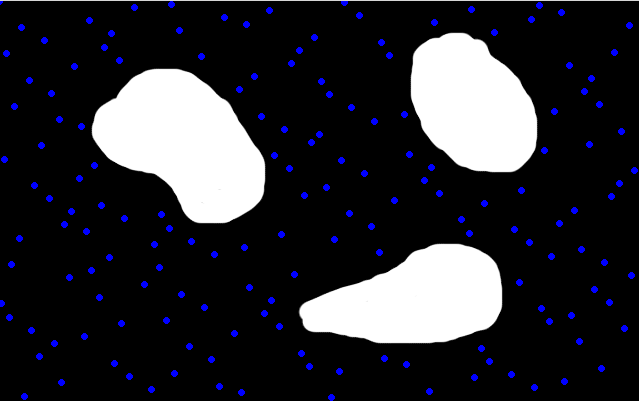
\includegraphics[width=\textwidth]{images/halton.png}
                \caption{Muestreo con puntos Halton}
                \label{fig:muestreo_halton}
        \end{subfigure}
        \caption{Comparativa de los distintos modos de muestreo del espacio libre}\label{fig:muestreo}
\end{figure}